\documentclass[xcolor=table]{beamer}

\usepackage[french]{babel}
\usepackage[latin1]{inputenc}
\usepackage[normalem]{ulem}
\usepackage[T1]{fontenc}
\usepackage{fancyhdr}   %% Pour la gestion des num�ros de page
\usepackage{graphicx}
\usepackage{amsmath}
\usepackage{mathrsfs}
\usepackage{amsfonts}
\usepackage{palatino}        %% Palatino fonts
\usepackage{mathptm}        %% PostScript Type 1 math fonts
\usepackage{dsfont} %% Pour mathds
\usepackage{color}
%%\usepackage{pstricks}
\usepackage{xmpmulti}
\usepackage{hyperref}
\usepackage{multimedia}
\usepackage{multirow}
%\usepackage[table]{xcolor}
\usepackage{fourier-orns}
\usepackage{subfigure}
\usepackage{tikz}

\DeclareMathAlphabet{\mathpzc}{OT1}{pzc}{m}{it}

\definecolor{vert}{rgb}{0.07,0.7,0.00}
\definecolor{gris}{gray}{0.70}
\definecolor{gris2}{gray}{0.95}
\definecolor{bleu}{rgb}{0.19,0.19,0.68}

%table setting
\newcommand\T{\rule{0pt}{2.6ex}}
\newcommand\B{\rule[-1.2ex]{0pt}{0pt}}
\renewcommand{\thesubfigure}{\thefigure.\arabic{subfigure}}

\usetheme{allee_marine} %voir fichier beaerthemeallee_marine.sty   ==> \usetheme{allee_marine}


%%%%%%%%%%%%%%%%%%%%%%%%%% Pr�sentation du document %%%%%%%%%%%%%%%%%%%%%%%%%%
\title[Master 1 Project]{Indexing big colored image bank : Texture 3.0}
\author[Etienne CAILLAUD, Thomas LE BRIS, Ibrahima GUEYE, Gaetan ADIER]{\textbf{Etienne CAILLAUD, Thomas LE BRIS, Ibrahima GUEYE, Gaetan ADIER}}
\institute [XLIM-SIC UMR CNRS 7252]{\textbf{XLIM-SIC Laboratory UMR CNRS 7252, Poitiers, France}}
\date{}

%%%%%%%%%%%%%%%%%%%%%%% Num�ro de pages en bas � gauche %%%%%%%%%%%%%%%%%%%%%%
\addtobeamertemplate{footline}{\color{blue}\hfill\insertframenumber/\inserttotalframenumber}

\pgfdeclareimage[height=96mm,width=128mm]{nombidon}{Fond}
\setbeamertemplate{background}{\pgfuseimage{nombidon}}

\pgfdeclareimage[height=96mm,width=128mm]{nombidon2}{Fond}
\setbeamertemplate{background}{\pgfuseimage{nombidon2}}

%%----------------------------------------------------------------------------
%% A chaque d�but de sous-section : g�n�re une table des mati�res
%%----------------------------------------------------------------------------
\AtBeginSection[]
{
   \setbeamertemplate{background}{\pgfuseimage{nombidon}}
   \begin{frame}<beamer>
    \frametitle{Outline}
    \tableofcontents[currentsection, hideallsubsections] %% affiche la section courante et les autres en gris�, masque les sous-sections
   \end{frame}
  \setbeamertemplate{background}{\pgfuseimage{nombidon2}}
}

\AtBeginSubsection[]
{
  \setbeamertemplate{background}{\pgfuseimage{nombidon}}
  \begin{frame}<beamer>
    \tableofcontents[sectionstyle=show/shaded,subsectionstyle=show/shaded/hide, subsubsectionstyle =hide]
  \end{frame}
   \setbeamertemplate{background}{\pgfuseimage{nombidon2}}
}

\AtBeginSubsubsection[]
{
  \setbeamertemplate{background}{\pgfuseimage{nombidon}}
  \begin{frame}<beamer>
    \tableofcontents[sectionstyle=show/shaded,subsectionstyle=show/shaded/hide,subsubsectionstyle =show/shaded/hide]
  \end{frame}
   \setbeamertemplate{background}{\pgfuseimage{nombidon2}}
}


%%%%%%%%%%%%%%%%%%%%%%%%%%%%%%%%%%%%%%%%%%%%%%%%%%%%%%%%%%%%%%%%%%%%%%%%%%%%%%
%%%%%%%%%%%%%%%%%%%%%%%%%%%%                       %%%%%%%%%%%%%%%%%%%%%%%%%%%
%%%%%%%%%%%%%%%%%%%%%%%%%%     D�BUT DU DOCUMENT     %%%%%%%%%%%%%%%%%%%%%%%%%
%%%%%%%%%%%%%%%%%%%%%%%%%%%%                       %%%%%%%%%%%%%%%%%%%%%%%%%%%
%%%%%%%%%%%%%%%%%%%%%%%%%%%%%%%%%%%%%%%%%%%%%%%%%%%%%%%%%%%%%%%%%%%%%%%%%%%%%%
\begin{document}
\graphicspath{{images/}}
\setbeamercolor{block title example}{bg = gray}

\begin{frame}
    \vspace{-1.5cm}
    \begin{tikzpicture}[remember picture,overlay]
        \node[xshift=0cm, above=8.6cm] at (current page.south west)
        {
\includegraphics[width=40cm,height=0.9cm]{cache_titre.png}};
        \node[xshift=2cm, above=2.8cm] at (current page.south west)
        {
\includegraphics[height=1.5cm]{Xlim.png}};
        \node[xshift=11cm, above=3cm] at (current page.south west)
        {
\includegraphics[height=1cm]{logo_une.jpg}};
        \node[xshift=6.5cm, above=0.7cm] at (current page.south west)
        {
\includegraphics[height=1.6cm]{Lifeclef.png}};
    \end{tikzpicture}
    \titlepage
\end{frame}

%%%%%%%%%%%%%%%%%%%%%%%%%%%%%%%%%%%%%%%%%%%%%%%%%%%%%%%%%%%%%%%%%%%%%%%%%%%%%%%%%%%%%%%%%%%%%%%%%%%%%
%%%%%%%%%%%                        D�but de la pr�sentation                       			 %%%%%%%%
%%%%%%%%%%%%%%%%%%%%%%%%%%%%%%%%%%%%%%%%%%%%%%%%%%%%%%%%%%%%%%%%%%%%%%%%%%%%%%%%%%%%%%%%%%%%%%%%%%%%%
\section{Introduction to the project context}
%%-----------------------------------------------------------------------------------------
%%-----------------------------------------------------------------------------------------
\begin{frame} \frametitle{Project context (1/3)}
%%-----------------------------------------------------------------------------------------
%% objective + image index
%%-----------------------------------------------------------------------------------------
\begin{block}{Objective}
  Test a solution for content based image indexing flaw : standard descriptors (SIFT, SURF, etc) lacking real color and texture information.
\end{block}
	
\begin{figure}
	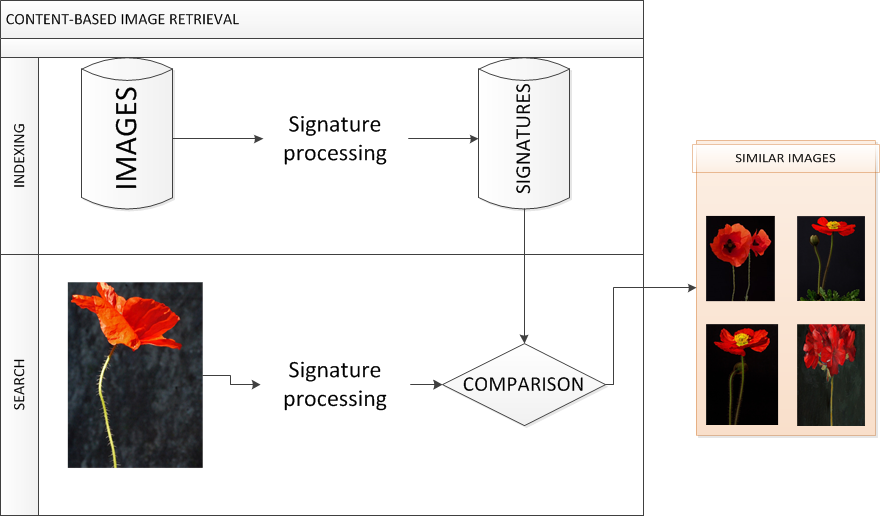
\includegraphics[scale=0.38]{CBIR.png}
\end{figure}



\end{frame}
%%-----------------------------------------------------------------------------------------

\begin{frame} \frametitle{Project context 2/3}
%%-----------------------------------------------------------------------------------------
%% Image Indexing
%%-----------------------------------------------------------------------------------------
\begin{block}{What is a descriptor ?}
	Algorithm applied to an image which output is a short vector
	of numbers which is invariant to common image transformations
	and can be compared with other descriptors in a	database.
\end{block}


\begin{figure}
   \begin{minipage}[c]{.56\linewidth}
      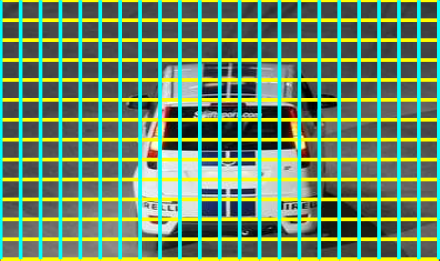
\includegraphics[scale=0.40]{dense_grid.png}
	  \caption{Densegrid}
   \end{minipage} \hfill
   \begin{minipage}[c]{.34\linewidth}
      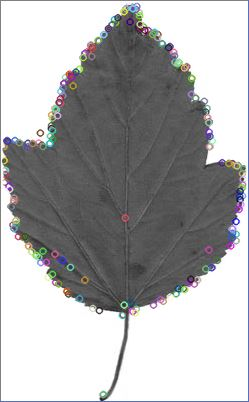
\includegraphics[scale=0.27]{siftKP.jpg}
	  \caption{Interest points}
   \end{minipage}
\end{figure}





\end{frame}
%%-----------------------------------------------------------------------------------------

\begin{frame} \frametitle{Project context 3/3}
%%-----------------------------------------------------------------------------------------
%% Parler de clef, des traitements couleurs marginaux ??}
%%-----------------------------------------------------------------------------------------
\begin{block}{What is a CLEF ?}
	International contest which purpose is to provide a place where labs and companies solution for multimedia analysis of life can compete against each other.
\end{block}

	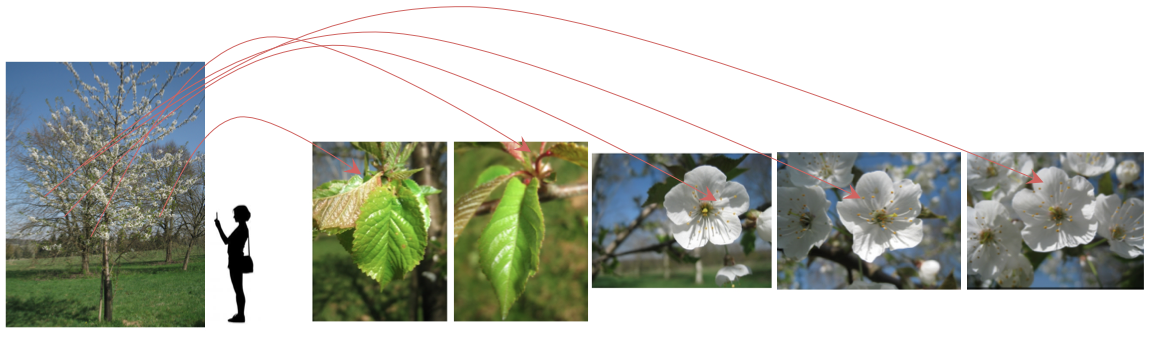
\includegraphics[scale=0.27]{OnePrunus.png}
\end{frame}
%%-----------------------------------------------------------------------------------------
%%-----------------------------------------------------------------------------------------

\begin{frame} \frametitle{Team presentation}
%%-----------------------------------------------------------------------------------------

% Schema demande par mr Richard
\begin{figure}[h]
    \center
    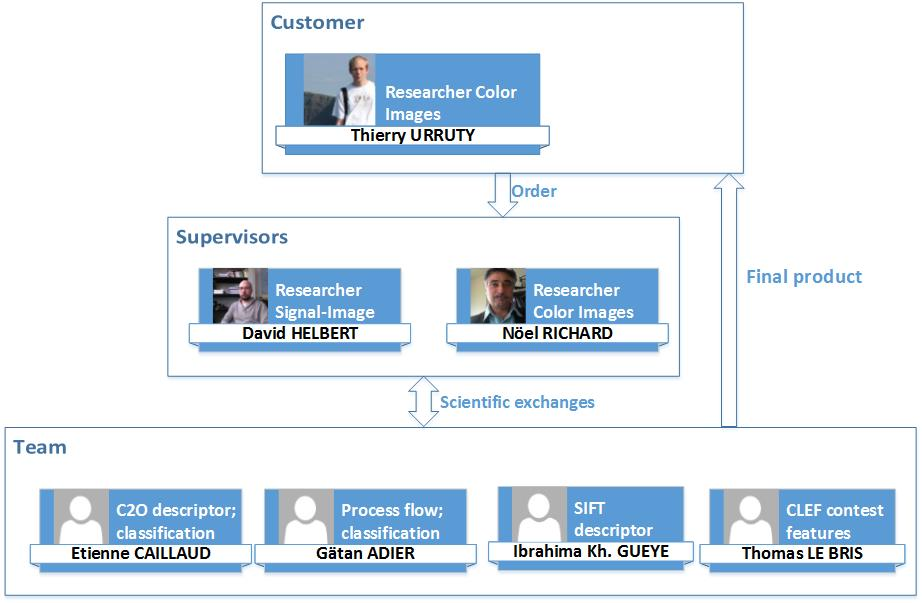
\includegraphics[scale=0.5]{Dessin1.jpg}
    \caption{Team}\label{fig:team}
\end{figure}

\end{frame}
%%-----------------------------------------------------------------------------------------


\begin{frame} \frametitle{User requirement}
%%-----------------------------------------------------------------------------------------

% Parler de la demande de base, ce qui etait convenu avec le client ...

\begin{itemize}
 \item Design  software programs:\\
   indexation of  images database,calculate descriptor according to  nature images
\item Adapt the last up to date designed color and texture attributes to the current image classification
\item Compare our results (using CLEF challenge metrics)
\item Provide an abstract of the comparisons and a technical report
\end{itemize}

\end{frame}
%%-----------------------------------------------------------------------------------------


\section{Work and results}
\begin{frame} \frametitle{SIFT(1/2)}

Key-points detection (x,y,$\sigma$)
\begin{itemize}

\item Scale-space extrema detection\\


\item  Key-point location\\


\item Orientation assignment\\


\item key-point descriptor
\\

\end{itemize}
\end{frame}

\begin{frame} \frametitle{SIFT(2/2)}
\begin{figure}[htbp]
    \begin{minipage}[c]{.45\linewidth}
      \begin{center}
	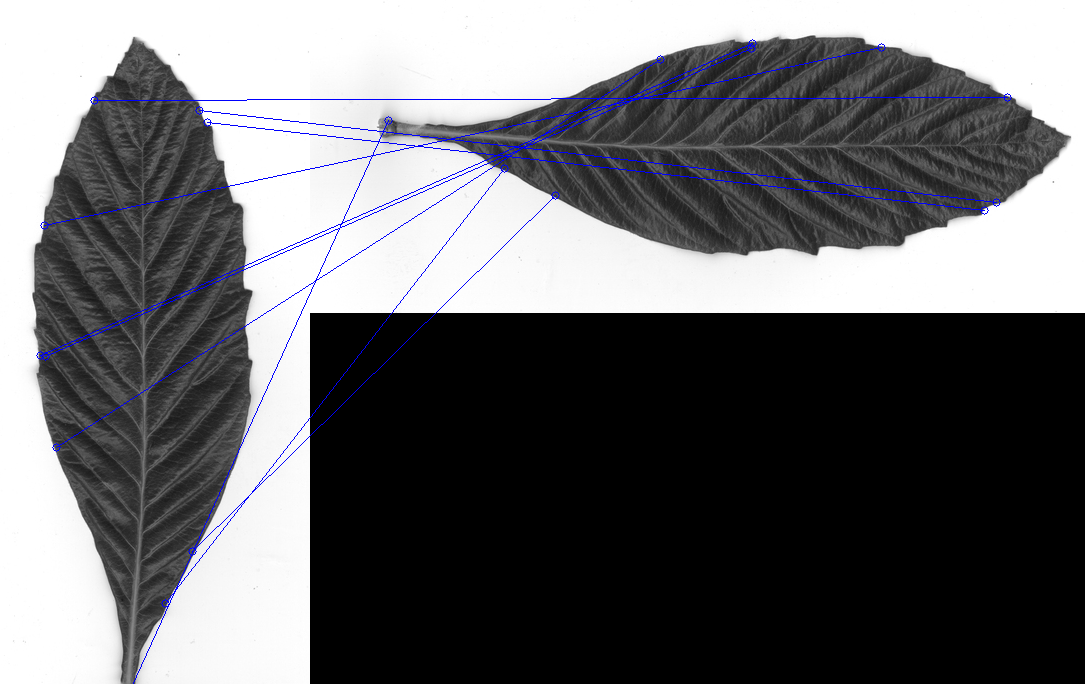
\includegraphics[scale=0.20]{Capture1.png}
	\caption{SIFT test1}
	\label{figure:Illustration}
      \end{center}
    \end{minipage}
    \hfill
    \begin{minipage}[c]{.45\linewidth}
      \begin{center}
	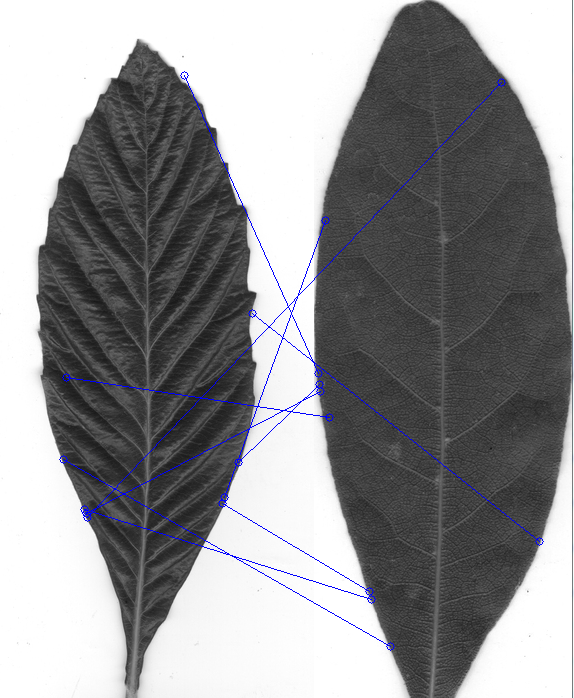
\includegraphics[scale=0.20]{Capture.png}
	\caption{SIFT test2}
	\label{figure:Illustration}
      \end{center}
    \end{minipage}
  \end{figure}
\end{frame}



\begin{frame} \frametitle{C$_2$O (1/4)}
%%-----------------------------------------------------------------------------------------
% Commencer par l'interet des C2O par rapport aux autres descripteurs, (difference entre traitement vectoriel et marginal,...)
   \begin{itemize}
        \item Limitation of marginal approach
        \item Necessity to get a vectorial treatment
        \item Include better texture and color informations
    \end{itemize}
\end{frame}
%%-----------------------------------------------------------------------------------------


\begin{frame} \frametitle{C$_2$O (2/4)}
%%-----------------------------------------------------------------------------------------
% Repprendre la premiere diapo en remplacant Lab par "perceptual space" et mettre les refs d'articles sur le lab en footnotes

\begin{itemize}
    \item Conversion to a perceptual space (adapted to human perception).
    \item C$_2$O matrix calculation.
    \item C$_2$O signature extraction.
\end{itemize}

\end{frame}
%%-----------------------------------------------------------------------------------------


\begin{frame} \frametitle{C$_2$O (3/4)}
%%-----------------------------------------------------------------------------------------
% Illustration de la difference de couleurs

\begin{itemize}
    \item Computation of the C$_2$O matrix by the color difference calculation
    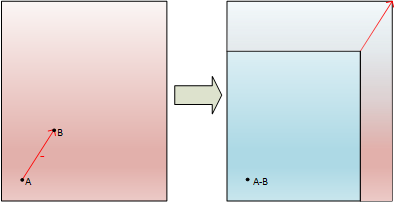
\includegraphics[scale=1.0]{ColorDiff.png}

\end{itemize}

\end{frame}
%%-----------------------------------------------------------------------------------------


\begin{frame} \frametitle{C$_2$O (3/4)}
%%-----------------------------------------------------------------------------------------

% Mettre des exemples de matrice C2O sur des images de la base qui seront parlant !!

\begin{itemize}


\item<1-> The C$_2$O matrix for a poorly textured image :
\only<1> {\begin{figure}[htbp]
    \begin{minipage}[c]{.40\linewidth}
      \begin{center}
    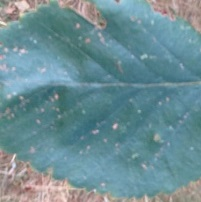
\includegraphics[scale=1.0]{61p.jpg}
    \caption{Image to characterize}
    \label{fig:Sig}
      \end{center}
    \end{minipage}
    \hfill
    \begin{minipage}[c]{.55\linewidth}
      \begin{center}
    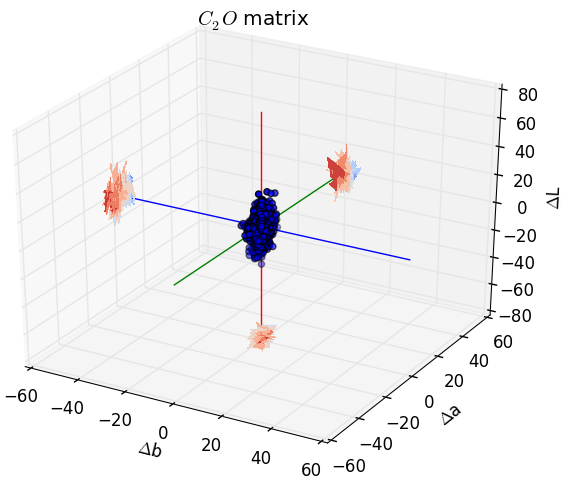
\includegraphics[scale=0.38]{C2OMat61p.png}
    \caption{Signature}
    \label{fig:Sig}
      \end{center}
    \end{minipage}
\end{figure}}
\item<2-> The C$_2$O matrix for a more textured image :
\only<2> {\begin{figure}[htbp]
    \begin{minipage}[c]{.40\linewidth}
      \begin{center}
    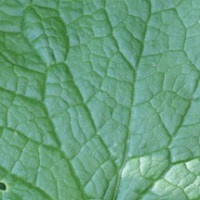
\includegraphics[scale=0.70]{119p.jpg}
    \caption{Image to characterize}
    \label{fig:Sig}
      \end{center}
    \end{minipage}
    \hfill
    \begin{minipage}[c]{.55\linewidth}
      \begin{center}
    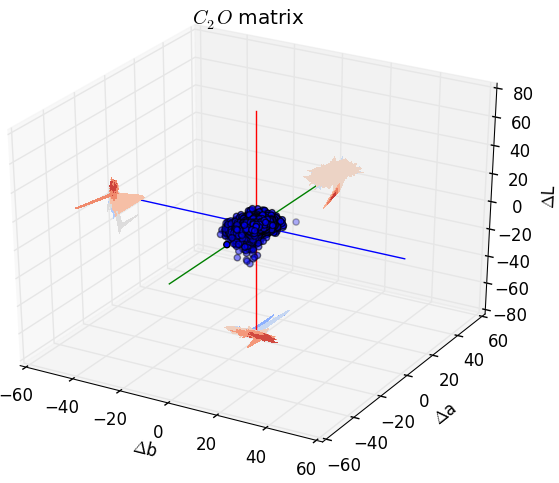
\includegraphics[scale=0.38]{C2OMat119p.png}
    \caption{Signature}
    \label{fig:Sig}
      \end{center}
    \end{minipage}
\end{figure}}
\item<3-> The C$_2$O matrix for a more textured and colored image :
\only<3> {\begin{figure}[htbp]
    \begin{minipage}[c]{.40\linewidth}
      \begin{center}
    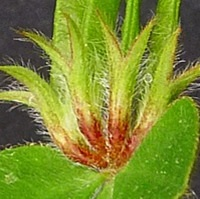
\includegraphics[scale=0.50]{97p.jpg}
    \caption{Image to characterize}
    \label{fig:Sig}
      \end{center}
    \end{minipage}
    \hfill
    \begin{minipage}[c]{.55\linewidth}
      \begin{center}
    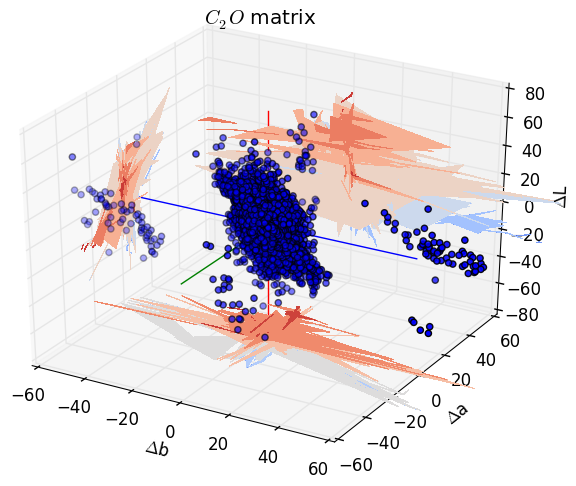
\includegraphics[scale=0.38]{C2OMat97p.png}
    \caption{Signature}
    \label{fig:Sig}
      \end{center}
    \end{minipage}
\end{figure}}

\end{itemize}

\end{frame}
%%-----------------------------------------------------------------------------------------


\begin{frame} \frametitle{C$_2$O (4/4)}
%%-----------------------------------------------------------------------------------------

% Mettre en petit en haut l'illustration coords spheriques et montrer les signatures correspondant aux matrices

\begin{tikzpicture}[remember picture, overlay]
  \node [anchor=north east, inner sep=4pt]  at (current page.north east)
     {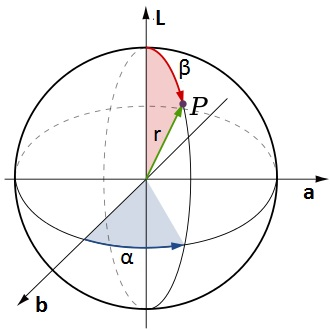
\includegraphics[height=3cm]{Spherical_Coordinates}};
\end{tikzpicture}



\begin{itemize}
\item<1-> The spherical quantization :
\only<1> {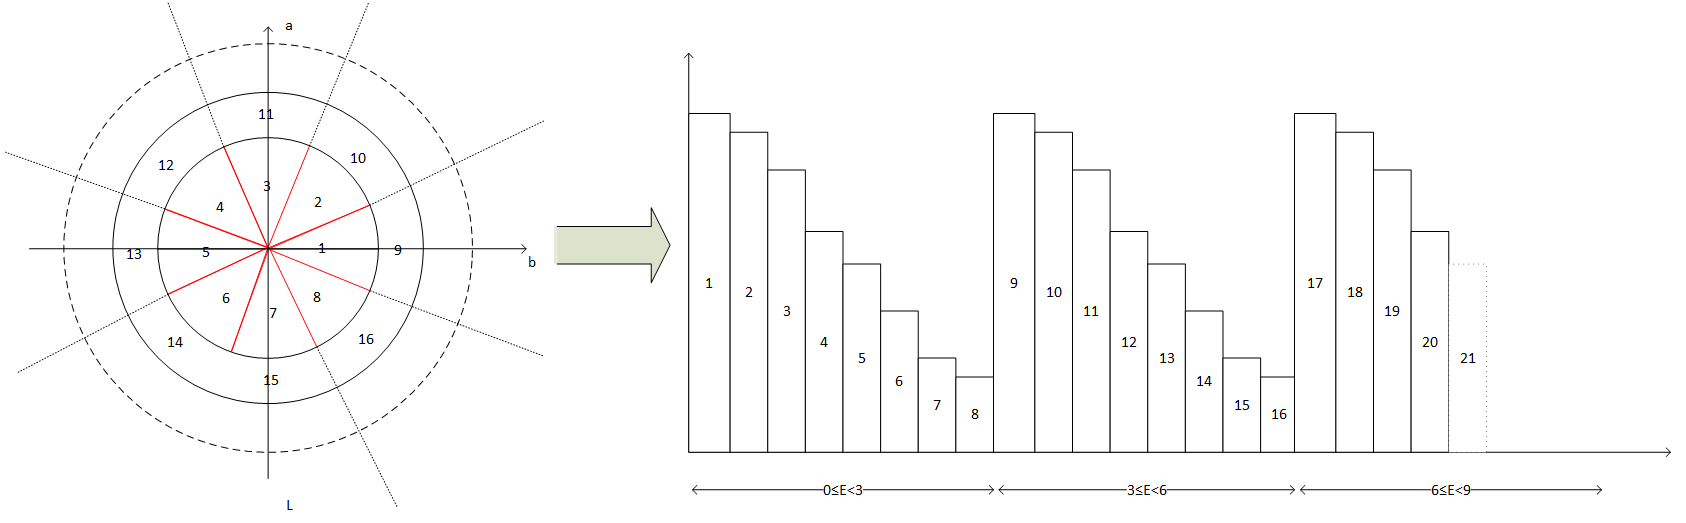
\includegraphics[height=3.4cm]{QuantificationSphericToHist.png}}
\item<2-> The C$_2$O signature for a poorly textured image :
\only<2> {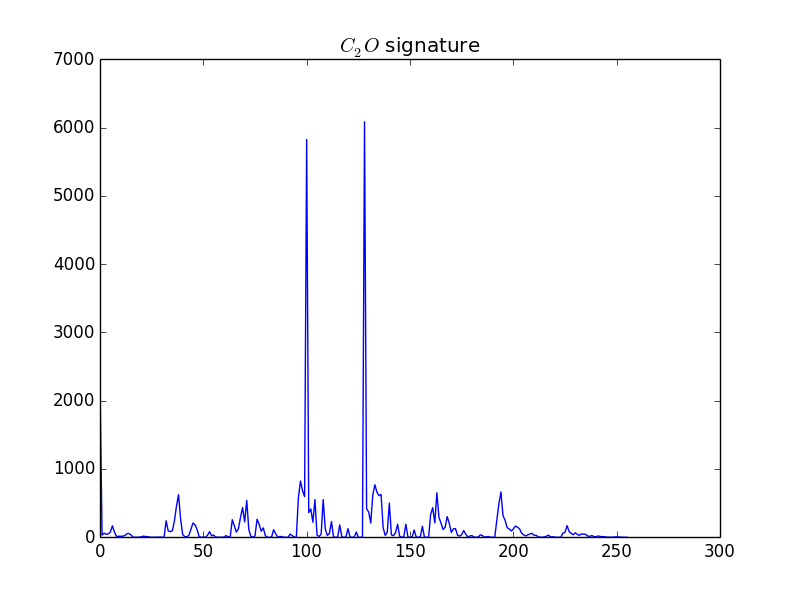
\includegraphics[height=4cm]{C2OSig61p.png}}
\item<3-> The C$_2$O signature for a more textured image :
\only<3> {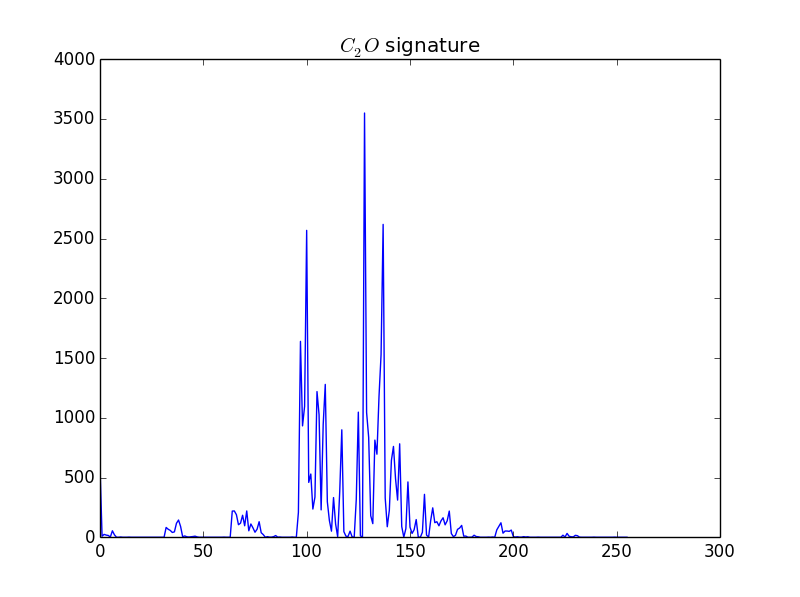
\includegraphics[height=4cm]{C2OSig119p.png}}
\item<4-> The C$_2$O signature for a more textured and colored image :
\only<4> {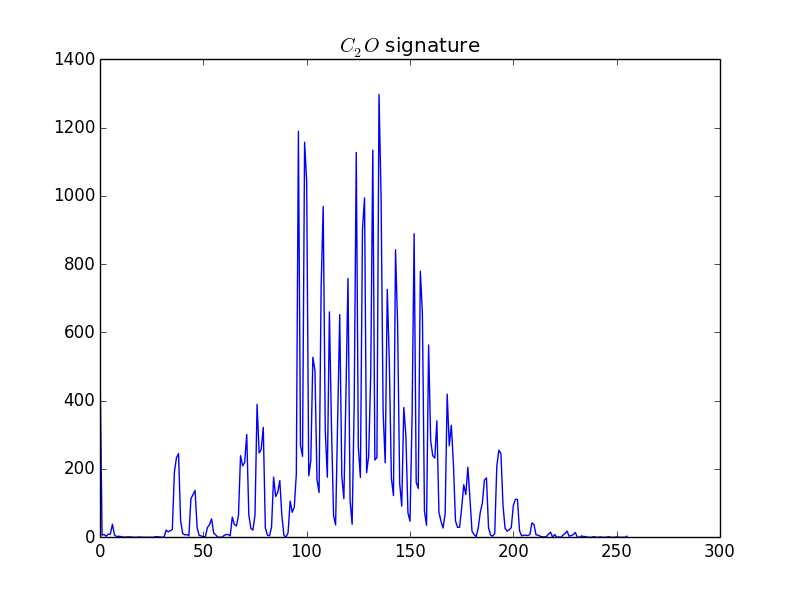
\includegraphics[height=4cm]{C2OSig97p.png}}

\end{itemize}



\end{frame}
%%-----------------------------------------------------------------------------------------




\begin{frame} \frametitle{Bag of word (1/2)}
%%-----------------------------------------------------------------------------------------
Reducing the number of points (100 in our case).

\begin{itemize}
    \item K-means
    \begin{itemize}
        \item Attribute the vectors to centroid vectors.
    \end{itemize}
\end{itemize}

\begin{figure}[h]
        \centering
        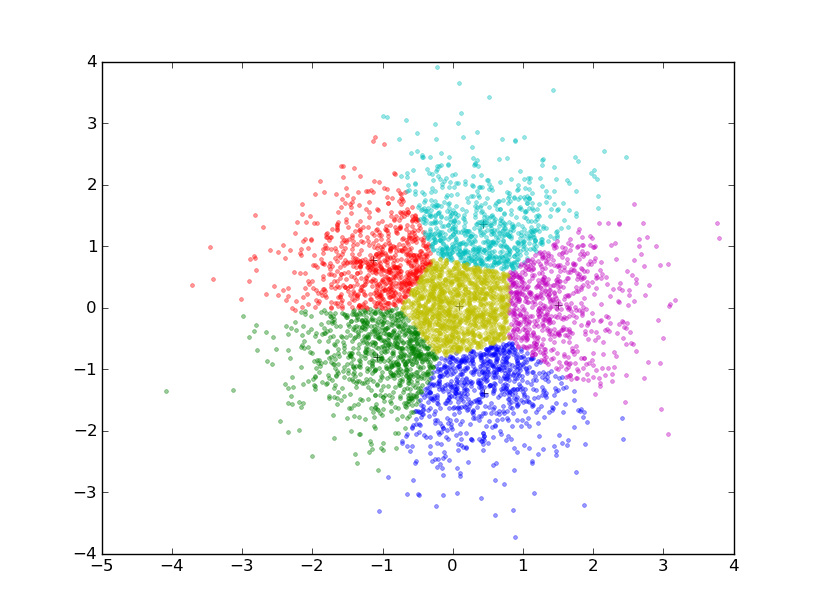
\includegraphics[scale=0.25]{k6n5000.png}
        \caption{K-means}
        \label{fig:kmeans}
    \end{figure}

\end{frame}
%%-----------------------------------------------------------------------------------------

\begin{frame} \frametitle{Bag of word (2/2)}
%%-----------------------------------------------------------------------------------------
\begin{itemize}
    \item Signature
    \begin{itemize}
        \item Design histogram in function of assignment of the vectors.
    \end{itemize}
\end{itemize}

\begin{figure}[htbp]
    \begin{minipage}[c]{.45\linewidth}
      \begin{center}
    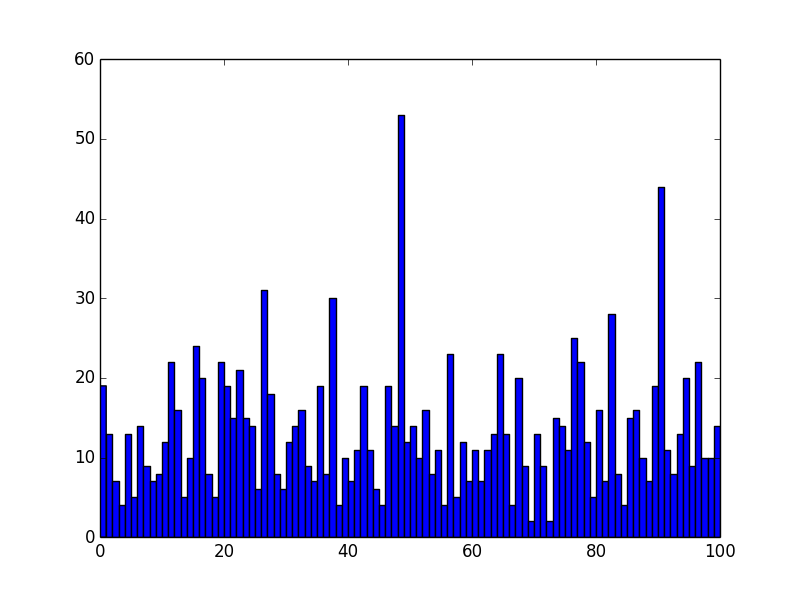
\includegraphics[scale=0.20]{131_sig.png}
    \caption{Signature 100 words - 1}
    \label{fig:image4}
      \end{center}
    \end{minipage}
    \hfill
    \begin{minipage}[c]{.45\linewidth}
      \begin{center}
    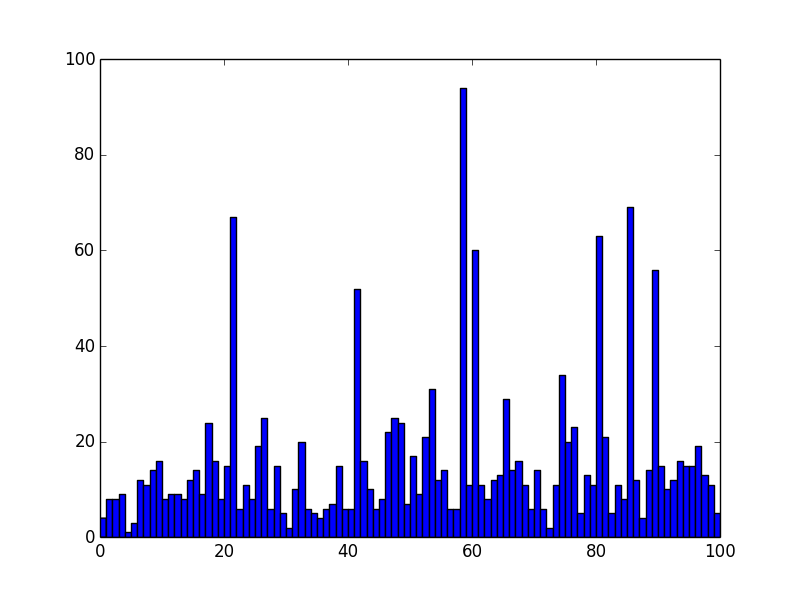
\includegraphics[scale=0.20]{132_sig.png}
    \caption{Signature 100 words - 2}
    \label{fig:image5}
      \end{center}
    \end{minipage}
\end{figure}


\end{frame}
%%-----------------------------------------------------------------------------------------


\begin{frame}\frametitle{K-nn(1/2)}

- The k nearest neighbor method

\begin{itemize}
\item<1-> Comparison to the dictionary .
\only<1> {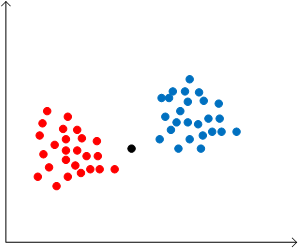
\includegraphics[height=4.2cm]{knnwc.png}} % Changer l'image
\only<2> {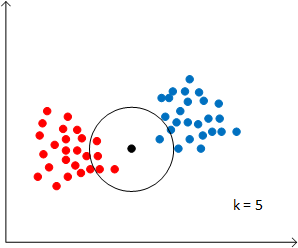
\includegraphics[height=4cm]{knnac.png}
\newline - 4 Occurrences of the 'red' class , - 1 occurrence of the 'blue' class \newline - The new point is attributed to the 'red' class}
\end{itemize}

\end{frame}

\begin{frame}\frametitle{K-nn(2/2)}

- Application for image classification

\begin{itemize}
\item More complex data.
\item Distances on signature vectors extracted from the K-mean method.
\item One most adapted distance type for each descriptor .
\end{itemize}

\end{frame}



\begin{frame} \frametitle{Results (1/2)}

\begin{itemize}
    \item Reduce data-base of 100 images composed of only 4 species.
\end{itemize}

  \begin{figure}[htbp]
    \begin{minipage}[c]{.45\linewidth}
      \begin{center}
	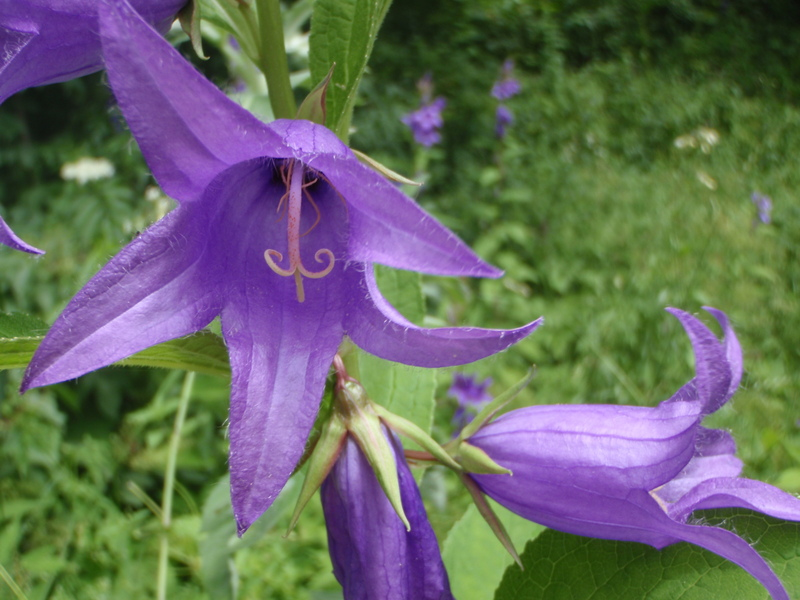
\includegraphics[scale=0.40]{63.jpg}
	\caption{First specie}
	\label{fig:image4}
      \end{center}
    \end{minipage}
    \hfill
    \begin{minipage}[c]{.45\linewidth}
      \begin{center}
	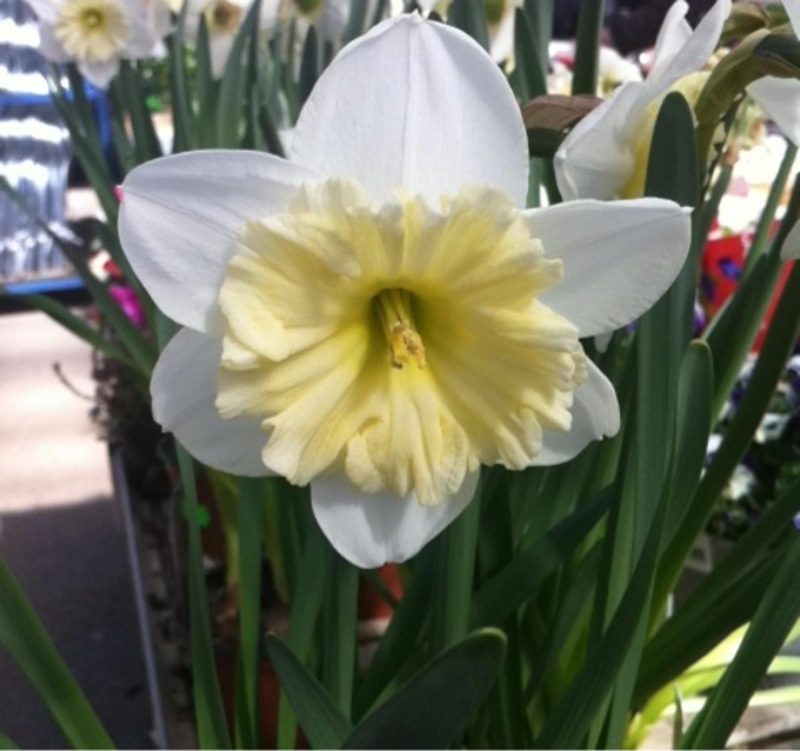
\includegraphics[scale=0.08]{2391.jpg}
	\caption{Second specie}
	\label{fig:image5}
      \end{center}
    \end{minipage}
  \end{figure}


  \begin{figure}[htbp]
    \begin{minipage}[c]{.45\linewidth}
      \begin{center}
	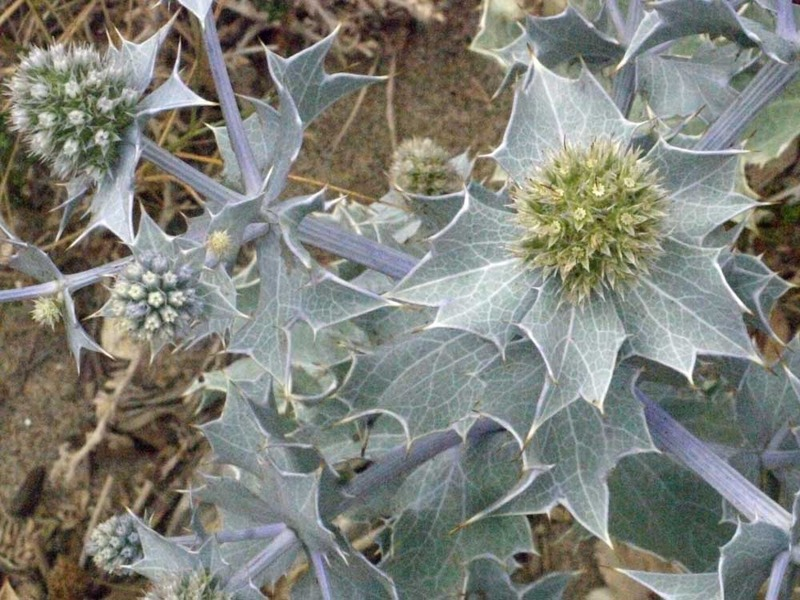
\includegraphics[scale=0.20]{4971.jpg}
	\caption{Third specie}
	\label{fig:image6}
      \end{center}
    \end{minipage}
    \hfill
    \begin{minipage}[c]{.45\linewidth}
      \begin{center}
	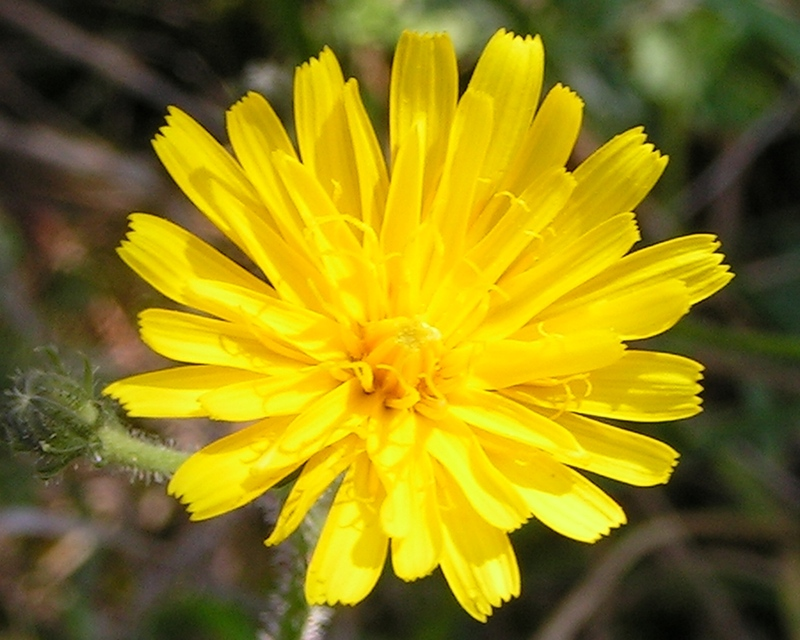
\includegraphics[scale=0.08]{21604.jpg}
	\caption{Fourth specie}
	\label{fig:image7}
      \end{center}
    \end{minipage}
  \end{figure}

\end{frame}


\begin{frame} \frametitle{Results (2/2)}
%%-----------------------------------------------------------------------------------------
\begin{itemize}
    \item Compare the two descriptors SIFT and C$_2$O.
\end{itemize}

\begin{figure}[htbp]
    \resizebox{3.5cm}{!}{
    \begin{minipage}[c]{.55\linewidth}
      \begin{center}
        \begin{table}[H]
        \centering
        \caption{SIFT result}
        \label{tab1}
        \begin{tabular}{|l|l|l|l|l|}
        \hline
        ID & Training Base & Test Base & Correct & Accuracy \\ \hline
        173 & 17 & 8 & 4 & 50\% \\ \hline
        1102 & 22 & 3 & 1 &\cellcolor{red!75} 33\% \\ \hline
        1889 & 16 & 9 & 1 & 11\% \\ \hline
        2717 & 15 & 10 & 7 &\cellcolor{red!75} 70\% \\ \hline
        Total & 70 & 30 & 9 & / \\ \hline
        \end{tabular}
        \end{table}
      \end{center}
    \end{minipage}}

    \resizebox{3.5cm}{!}{
    \begin{minipage}[c]{.55\linewidth}
      \begin{center}
            \begin{table}[H]
            \caption{C$_2$O result}
            \label{tab2}
            \begin{tabular}{|l|l|l|l|l|}
            \hline
            ID & Training Base & Test Base & Correct & Accuracy \\ \hline
            173 & 17 & 8 & 1 & 12.5\% \\ \hline
            1102 & 22 & 3 & 1 &\cellcolor{red!75} 33\% \\ \hline
            1889 & 16 & 9 & 0 & 0\% \\ \hline
            2717 & 15 & 10 & 7 &\cellcolor{red!75} 70\% \\ \hline
            Total & 70 & 30 & 9 & / \\ \hline
            \end{tabular}
            \end{table}
      \end{center}
    \end{minipage}}
\end{figure}

\end{frame}
%%-----------------------------------------------------------------------------------------

\begin{frame} \frametitle{Discussion}

\begin{itemize}
    \item Classification
    \vspace{0.3cm}
    \begin{itemize}
        \item To much reducing on the K-means (100 words).
        \vspace{0.15cm}
        \item Euclidean distance not the most efficient or adapt.
    \end{itemize}
    \vspace{0.7cm}
    \item C$_2$O
    \vspace{0.3cm}
    \begin{itemize}
        \item The concatenation way is not optimal.
        \item Parameters D, alpha, and beta has to be discussed regarding to the images.
    \end{itemize}
\end{itemize}
\end{frame}
%%-----------------------------------------------------------------------------------------


%%-----------------------------------------------------------------------------------------
\section{Project management}
%%-----------------------------------------------------------------------------------------




\begin{frame} \frametitle{Scheduling (1/2)}
%%-----------------------------------------------------------------------------------------
% Montrer le passage d'un gantt a un backlog produit, => mettre l'accent sur la modification du gantt sans modification du backlog notable

\begin{itemize}
\item The previsional forecast Gantt chart  :
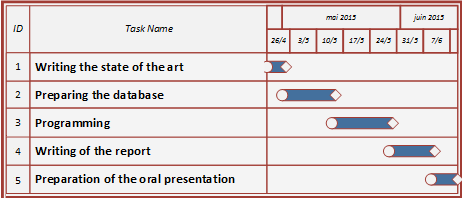
\includegraphics[scale=0.40]{GanttPrez.png}
\item All time affectation done before the beginning of the project
\item Rarely respected in important project
\end{itemize}

\end{frame}
%%-----------------------------------------------------------------------------------------


\begin{frame} \frametitle{Scheduling (2/2)}
%%-----------------------------------------------------------------------------------------
% Montrer le passage d'un gantt a un backlog produit, => mettre l'accent sur la modification du gantt sans modification du backlog notable


\begin{itemize}
\item The project backlog  :
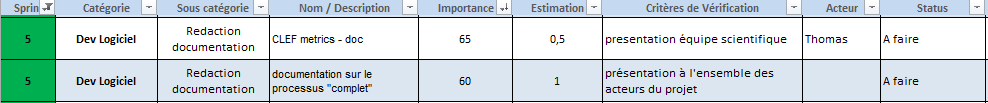
\includegraphics[scale=0.30]{backlog.png}
\item Allow to change the affectation of a task
\item Weekly time affectation : could be adapted to unforeseen
\end{itemize}


\end{frame}
%%-----------------------------------------------------------------------------------------


\begin{frame} \frametitle{Our experience}
%%-----------------------------------------------------------------------------------------
% Complique? Utile ?
\begin{itemize}
\item Minimal lack of time
\item The possibility of changing task affectation is really useful
\item An adaptation of the initial schedule has been realised
\end{itemize}

\end{frame}
%%-----------------------------------------------------------------------------------------



%%-----------------------------------------------------------------------------------------
\section{Conclusion}
%%-----------------------------------------------------------------------------------------


\begin{frame} \frametitle{Objectives}
%%-----------------------------------------------------------------------------------------

% Rappel des objectifs de base
\end{frame}
%%-----------------------------------------------------------------------------------------


\begin{frame} \frametitle{Achieved work}
%%-----------------------------------------------------------------------------------------

% Rappel des objectifs de base
\end{frame}
%%-----------------------------------------------------------------------------------------


\begin{frame} \frametitle{Problem encountered}
%%-----------------------------------------------------------------------------------------

% Rappel des objectifs de base
\end{frame}
%%-----------------------------------------------------------------------------------------


\begin{frame} \frametitle{Personal point of view}
%%-----------------------------------------------------------------------------------------

% Rappel des objectifs de base
\end{frame}
%%-----------------------------------------------------------------------------------------






\section{}
\begin{frame}\frametitle{}
%%-----------------------------------------------------------------------------------------
    \begin{center}
        Thanks for attention
    \end{center}
\end{frame}
%%-----------------------------------------------------------------------------------------


\end{document}

